\documentclass{math}

\usepackage{graphicx}
\usepackage{listings}
\lstset{basicstyle=\ttfamily\footnotesize,breaklines=true}
\geometry{letterpaper, margin=0.8in}

\title{CSCI 251: Concepts of Parallel and Distributed Systems}
\author{Alvin Lin}
\date{September 2017 - December 2017}

\begin{document}

\maketitle

\section*{Project 1}
This project involved the implementation of a serial and parallel bitonic sort.
This implementation was done serially in C and parallelized using POSIX threads.
The parallel implementation of the algorithm simply divided the recursive
operation among the specified number of threads.

\subsection*{Serial Psuedocode}
This implementation assumed that the given data elements to sort were integers
and that the size of the data set was a power of two. In addition, it also
assumes that the number of threads to distribute this among is a power of two.
\begin{lstlisting}
penis
\end{lstlisting}

\subsection*{Analysis}
The full data sheet of the runtimes is in the included data.pdf file.
In general, the runtime improved the more threads we used.
\begin{center}
  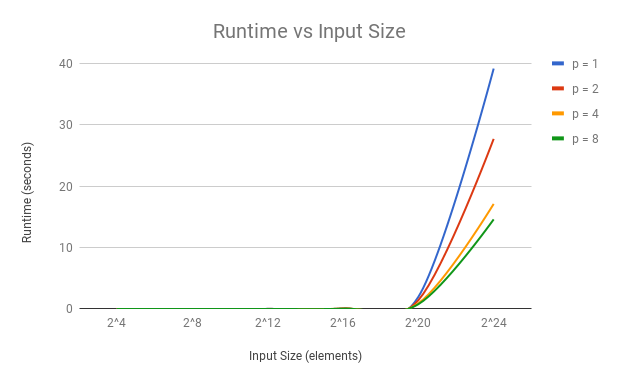
\includegraphics[width=16cm]{assets/project2_runtime.png}
\end{center}
At low data sizes though, the extra threads caused overhead and led to a
decrease in speedup. In general however, more threads allowed for better
performance at high input sizes.
\begin{center}
  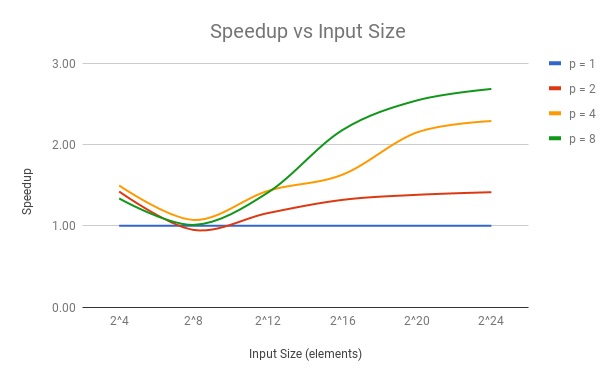
\includegraphics[width=16cm]{assets/project2_speedup.png}
\end{center}


\end{document}
